\documentclass[11pt, a4paper]{article}
\usepackage[utf8]{inputenc}
\usepackage[T1]{fontenc}
\usepackage[swedish]{babel}
\usepackage{geometry}
\usepackage{setspace}
\usepackage{csquotes}
\usepackage{natbib}
\usepackage{url}
\usepackage{tikz}
\usepackage{textcomp}
\usepackage{newunicodechar}
\newunicodechar{—}{---}


\newunicodechar{→}{$\rightarrow$}
\usetikzlibrary{arrows.meta, positioning, shapes.misc, fit}

\geometry{margin=2.5cm}
\onehalfspacing

\title{Forskningsläge och Referensram \\[4pt]
\large PhD-ansökan i Datavetenskap: \\ Data-driven produktutveckling, produktförbättring och produktledning}
\author{Rickard Åberg}
\date{\today}

\begin{document}



\section*{Forskningsläge}
Under de senaste åren har mjukvaruintensiva företag genomgått en omfattande digital transformation där
data och artificiell intelligens (AI) spelar en allt viktigare roll i produktutvecklingen.
\citet{bosch2019speed} och \citet{holmstrom2022data} betonar att företag behöver integrera
kontinuerlig datainsamling, analys och modelluppdatering i hela produktlivscykeln.
Detta kräver nya processer, ofta benämnda \textit{DataOps} och \textit{MLOps}, som möjliggör att dataflöden,
modellträning och distribution hanteras med samma grad av automatisering och spårbarhet som inom traditionell DevOps.

\citet{holmstrom2020ai} introducerar ett ramverk för att bedöma AI-mognad i företag,
vilket innefattar organisatorisk beredskap, teknisk infrastruktur och kulturell anpassning.
I industrin har dessa idéer operationaliserats genom
kontinuerliga experiment, datadrivna beslut och återkoppling från produkter i drift
\citep{bosch2018data}.
Trots framsteg kvarstår utmaningar kring datakvalitet, etik, ansvarsfördelning och
modellunderhåll över tid.

\section*{Syfte och forskningsfrågor}
Syftet med det föreslagna projektet är att undersöka hur principerna för
DataOps och MLOps kan tillämpas inom industriell produktutveckling för att stödja
kontinuerligt lärande och AI-drivna beslut.
Projektet avser att bidra till förståelsen av hur organisationer kan strukturera sina
data- och modellflöden på ett sätt som gynnar både teknisk kvalitet och affärsvärde.


\begin{figure}[h!]
\centering
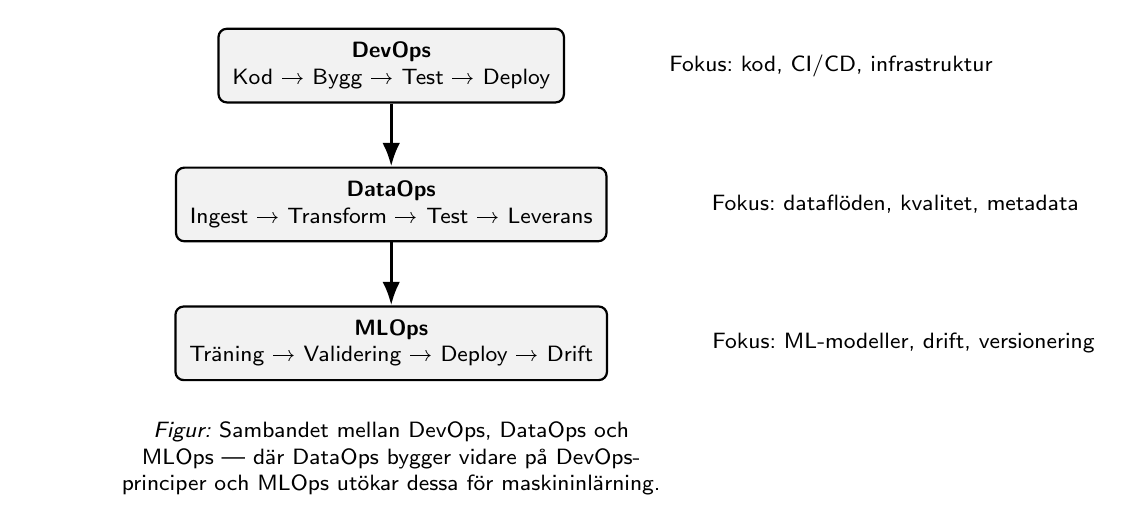
\begin{tikzpicture}[
  font=\sffamily\footnotesize,
  box/.style={rounded corners=3pt, draw, thick, inner sep=5pt, minimum width=30mm, align=center},
  arrow/.style={-{Latex[length=3mm]}, very thick}
]

% Main boxes
\node[box, fill=gray!10] (devops) { \textbf{DevOps}\\Kod → Bygg → Test → Deploy };
\node[box, fill=gray!10, below=8mm of devops] (dataops) { \textbf{DataOps}\\Ingest → Transform → Test → Leverans };
\node[box, fill=gray!10, below=8mm of dataops] (mlops) { \textbf{MLOps}\\Träning → Validering → Deploy → Drift };

% Arrows
\draw[arrow] (devops) -- (dataops);
\draw[arrow] (dataops) -- (mlops);

% Side labels
\node[right=12mm of devops.east, align=left] {Fokus: kod, CI/CD, infrastruktur};
\node[right=12mm of dataops.east, align=left] {Fokus: dataflöden, kvalitet, metadata};
\node[right=12mm of mlops.east, align=left] {Fokus: ML-modeller, drift, versionering};

% Caption under
\node[below=4mm of mlops.south, align=center, text width=9cm]
  {\emph{Figur:} Sambandet mellan DevOps, DataOps och MLOps — där DataOps bygger vidare på DevOps-principer och MLOps utökar dessa för maskininlärning.};

\end{tikzpicture}
\end{figure}


\textbf{Exempel på forskningsfrågor:}
\begin{itemize}
    % \item Hur kan DataOps- och MLOps-principer integreras i befintliga produktutvecklingsprocesser?
    % \item Vilka tekniska och organisatoriska hinder uppstår vid införandet av datadrivna arbetssätt?
    % \item Hur kan kontinuerlig återkoppling från användardata bidra till produktförbättring och innovation?
    % De huvudsakliga forskningsfrågorna för projektet är:

 \item Vilken är rollen och användningen av data i utvecklingen av mjukvaruintensiva inbyggda system?

 \item Vilka tillvägagångssätt och arkitekturer krävs för att möjliggöra datadriven utveckling av       mjukvaruintensiva inbyggda system?
 
 \item Hur förändras och ersätts nuvarande roller och arbetssätt genom införandet av nya metoder (såsom DevOps, DataOps och MLOps) samt genom användning av digitala teknologier (mjukvara, data och artificiell intelligens)?

\end{itemize}

\section*{Metodologisk ansats}
Projektet planeras som en kombination av empiriska fallstudier i samarbete med industripartners
och teoretisk modellering av data- och modellflöden.
Den empiriska delen kan inkludera observationer, intervjuer och analys av befintliga DevOps- och MLOps-miljöer.
Resultaten kan sedan användas för att formulera designprinciper och riktlinjer
för datadriven produktutveckling.

\bibliographystyle{apalike}
\bibliography{referenser}

\end{document}
